\documentclass[a4paper,12pt]{article}
%All Layout Packages are defined in the Header.tex
\usepackage[utf8]{inputenc}
\usepackage[english]{babel}
\usepackage{fancyhdr}

%This is to print solutions or not
\usepackage{ifthen}

%This is to include src code
\usepackage{listings}
\lstset{ %
  backgroundcolor=\color{white},   % choose the background color; you must add \usepackage{color} or \usepackage{xcolor}
  basicstyle=\footnotesize,        % the size of the fonts that are used for the code
  breakatwhitespace=false,         % sets if automatic breaks should only happen at whitespace
  breaklines=true,                 % sets automatic line breaking
  captionpos=b,                    % sets the caption-position to bottom
  commentstyle=\color{commentsColor}\textit,    % comment style
  deletekeywords={...},            % if you want to delete keywords from the given language
  escapeinside={\%*}{*)},          % if you want to add LaTeX within your code
  extendedchars=true,              % lets you use non-ASCII characters; for 8-bits encodings only, does not work with UTF-8
  frame=tb,	                   	   % adds a frame around the code
  keepspaces=true,                 % keeps spaces in text, useful for keeping indentation of code (possibly needs columns=flexible)
  keywordstyle=\color{keywordsColor}\bfseries,       % keyword style
  language=Python,                 % the language of the code (can be overrided per snippet)
  otherkeywords={*,...},           % if you want to add more keywords to the set
  numbers=left,                    % where to put the line-numbers; possible values are (none, left, right)
  numbersep=5pt,                   % how far the line-numbers are from the code
  numberstyle=\tiny\color{commentsColor}, % the style that is used for the line-numbers
  rulecolor=\color{black},         % if not set, the frame-color may be changed on line-breaks within not-black text (e.g. comments (green here))
  showspaces=false,                % show spaces everywhere adding particular underscores; it overrides 'showstringspaces'
  showstringspaces=false,          % underline spaces within strings only
  showtabs=false,                  % show tabs within strings adding particular underscores
  stepnumber=1,                    % the step between two line-numbers. If it's 1, each line will be numbered
  stringstyle=\color{stringColor}, % string literal style
  tabsize=2,	                   % sets default tabsize to 2 spaces
  title=\lstname,                  % show the filename of files included with \lstinputlisting; also try caption instead of title
  columns=fixed                    % Using fixed column width (for e.g. nice alignment)
}


%Use this to customize margins
\usepackage[
  top=2cm,
  bottom=2cm,
  left=1cm,
  right=1cm,
  headheight=17pt, % as per the warning by fancyhdr
  includehead,includefoot,
  heightrounded, % to avoid spurious underfull messages
]{geometry} 

%Use this to customize headers
\pagestyle{fancy}
\fancyhf{}
\fancyhead[LE,RO]{Version: \today}
\fancyhead[RE,LO]{Geophysics Exercises}
\fancyfoot[CE,CO]{\leftmark}
\fancyfoot[LE,RO]{\thepage}
\usepackage{graphicx}
\renewcommand{\headrulewidth}{2pt}
\renewcommand{\footrulewidth}{1pt}


%Use this to customize tables
\usepackage[table]{xcolor}
\usepackage{tabularx}
\usepackage{booktabs}


\setlength{\arrayrulewidth}{1mm}
\setlength{\tabcolsep}{18pt}
\renewcommand{\arraystretch}{1.5}


%Use this to customize colors
\definecolor{myblue}{rgb}{0.0, 0.53, 0.74}
\definecolor{myred}{rgb}{1.0, 0.8, 0.89}
\definecolor{babyblueeyes}{rgb}{0.63, 0.79, 0.95}
\definecolor{beaublue}{rgb}{0.74, 0.83, 0.9}
\definecolor{bluegray}{rgb}{0.4, 0.6, 0.8}
\definecolor{commentsColor}{rgb}{0.497495, 0.497587, 0.497464}
\definecolor{keywordsColor}{rgb}{0.000000, 0.000000, 0.635294}
\definecolor{stringColor}{rgb}{0.558215, 0.000000, 0.135316}
\definecolor{burgundy}{rgb}{0.5, 0.0, 0.13}
%Here some pre-defined commands
\newcommand{\ProtocolTable}[6]
{
\begin{table}[]
\begin{tabular}{|p{1.8cm} p{3.8cm} p{1.8cm} p{2.0cm}|}
\hline
 \rowcolor{beaublue}\textbf{Name}:&\multicolumn{3}{l}{#1} \\
 \rowcolor{beaublue}\textbf{Folder:}&\multicolumn{3}{l}{#2} \\
 \rowcolor{beaublue}\textbf{Instrument:}&#3&\textbf{Date:}&#4 \\
  \rowcolor{beaublue}\textbf{Operator:}&#5&\textbf{Location:}&#6\\
\hline
\end{tabular}
\end{table}
}
\usepackage{enumitem}
\usepackage{blindtext}
\usepackage{afterpage}
\usepackage{lipsum,lmodern}
\usepackage[most]{tcolorbox}
\tcbuselibrary{skins}
\usepackage{hyperref}

%no indents at paragraphs 
\setlength\parindent{0pt}

%% Oh yes. TIKZ pictures / graphs
%% -------------------------------------
\usepackage{tikz}
\usepackage{pgfplots}
\usepackage{tikz-3dplot}
\usetikzlibrary{calc,fadings,decorations.pathreplacing,shadings,intersections}



%Start the document here.
\begin{document}
\section{Exercises for Gravimetry}
\subsection{The shell theorem}
\subsection{Gravitational potential inside and outside a sphere with constant density}
\subsection{Detection of a spherical object in the sub-surface}
\textbf{(a)} In the lecture we have discussed the general shape of a gravity anomaly for a sphere with radius $R$ located at depth $z$ below the surface. Formulate the problem in a relative sense using density contrasts ($\Delta \rho$). Derive an analytical expression for the vertical anomaly as a function of the lateral distance $x$ and depth $z$. Calculate the maximum anomalies that you would expect for some realistic settings (e.g., a limestone cave.)\\

\noindent\fcolorbox{myblue}{lightgray}{\parbox{\textwidth}{
\textbf{Solution:} Because we have a spherical object, there is not much difference to the point mass scenario discussed in class. The gravitational force exhibited by the sphere is:
$$
\vec{g} = G\frac{M}{r^2}\hat{r}
$$
The mass anomaly $M$ (formulated in a relative sense) of the sphere is given by:
$$
M = \frac{4}{3}\pi R^3 \Delta \rho
$$
At distance $x$ the distance to the sphere is $r=\sqrt{x^2+z^2}$. The gravimeter only measures the vertical component of $\vec{g}$:
$$
g_z = |\vec{g}|\sin\alpha = |\vec{g}|\frac{z}{r}
$$
% \begin{center}
% \includegraphics[width=0.5\textwidth]{SphereSketch.png}
% \end{center}

which brings us to:
\begin{align*}
g_z &= \frac{4}{3}\pi R^3 \Delta \rho \frac{G}{r^2} \frac{z}{r} \\
&= \frac{4}{3}\pi R^3 \Delta \rho \frac{G}{r^3} z \\
& = \frac{4}{3}\pi R^3 \Delta \rho G \frac{z}{(x^2+z^2)^\frac{3}{2}}
\end{align*}
We will encounter the maximum value of the anomaly at $x = 0$ (directly above the target):
$$
g_{z,max} = \frac{4}{3}\pi R^3 \Delta \rho G \frac{1}{z^2}
$$
which for the limestone cave example is approximately -0.35 mGal (see below).
}}
\pagebreak


\noindent \textbf{(b)} Use a piece of software of your choice (e.g., Excel, SciDAVis, Matlab, Python) and plot the expected vertical gravity anomaly for a specific setting as a function of lateral distance $x$. Visualize how this profile changes as you vary, e.g., the depth of the object. Label your axis and post a picture in the forum alongside with a comment which software you used.


\lstinputlisting[language=matlab]{../Src/Exercises/Gravimetry/Gravimetry01.m}
%\end{lstlisting}
% \begin{center}
% 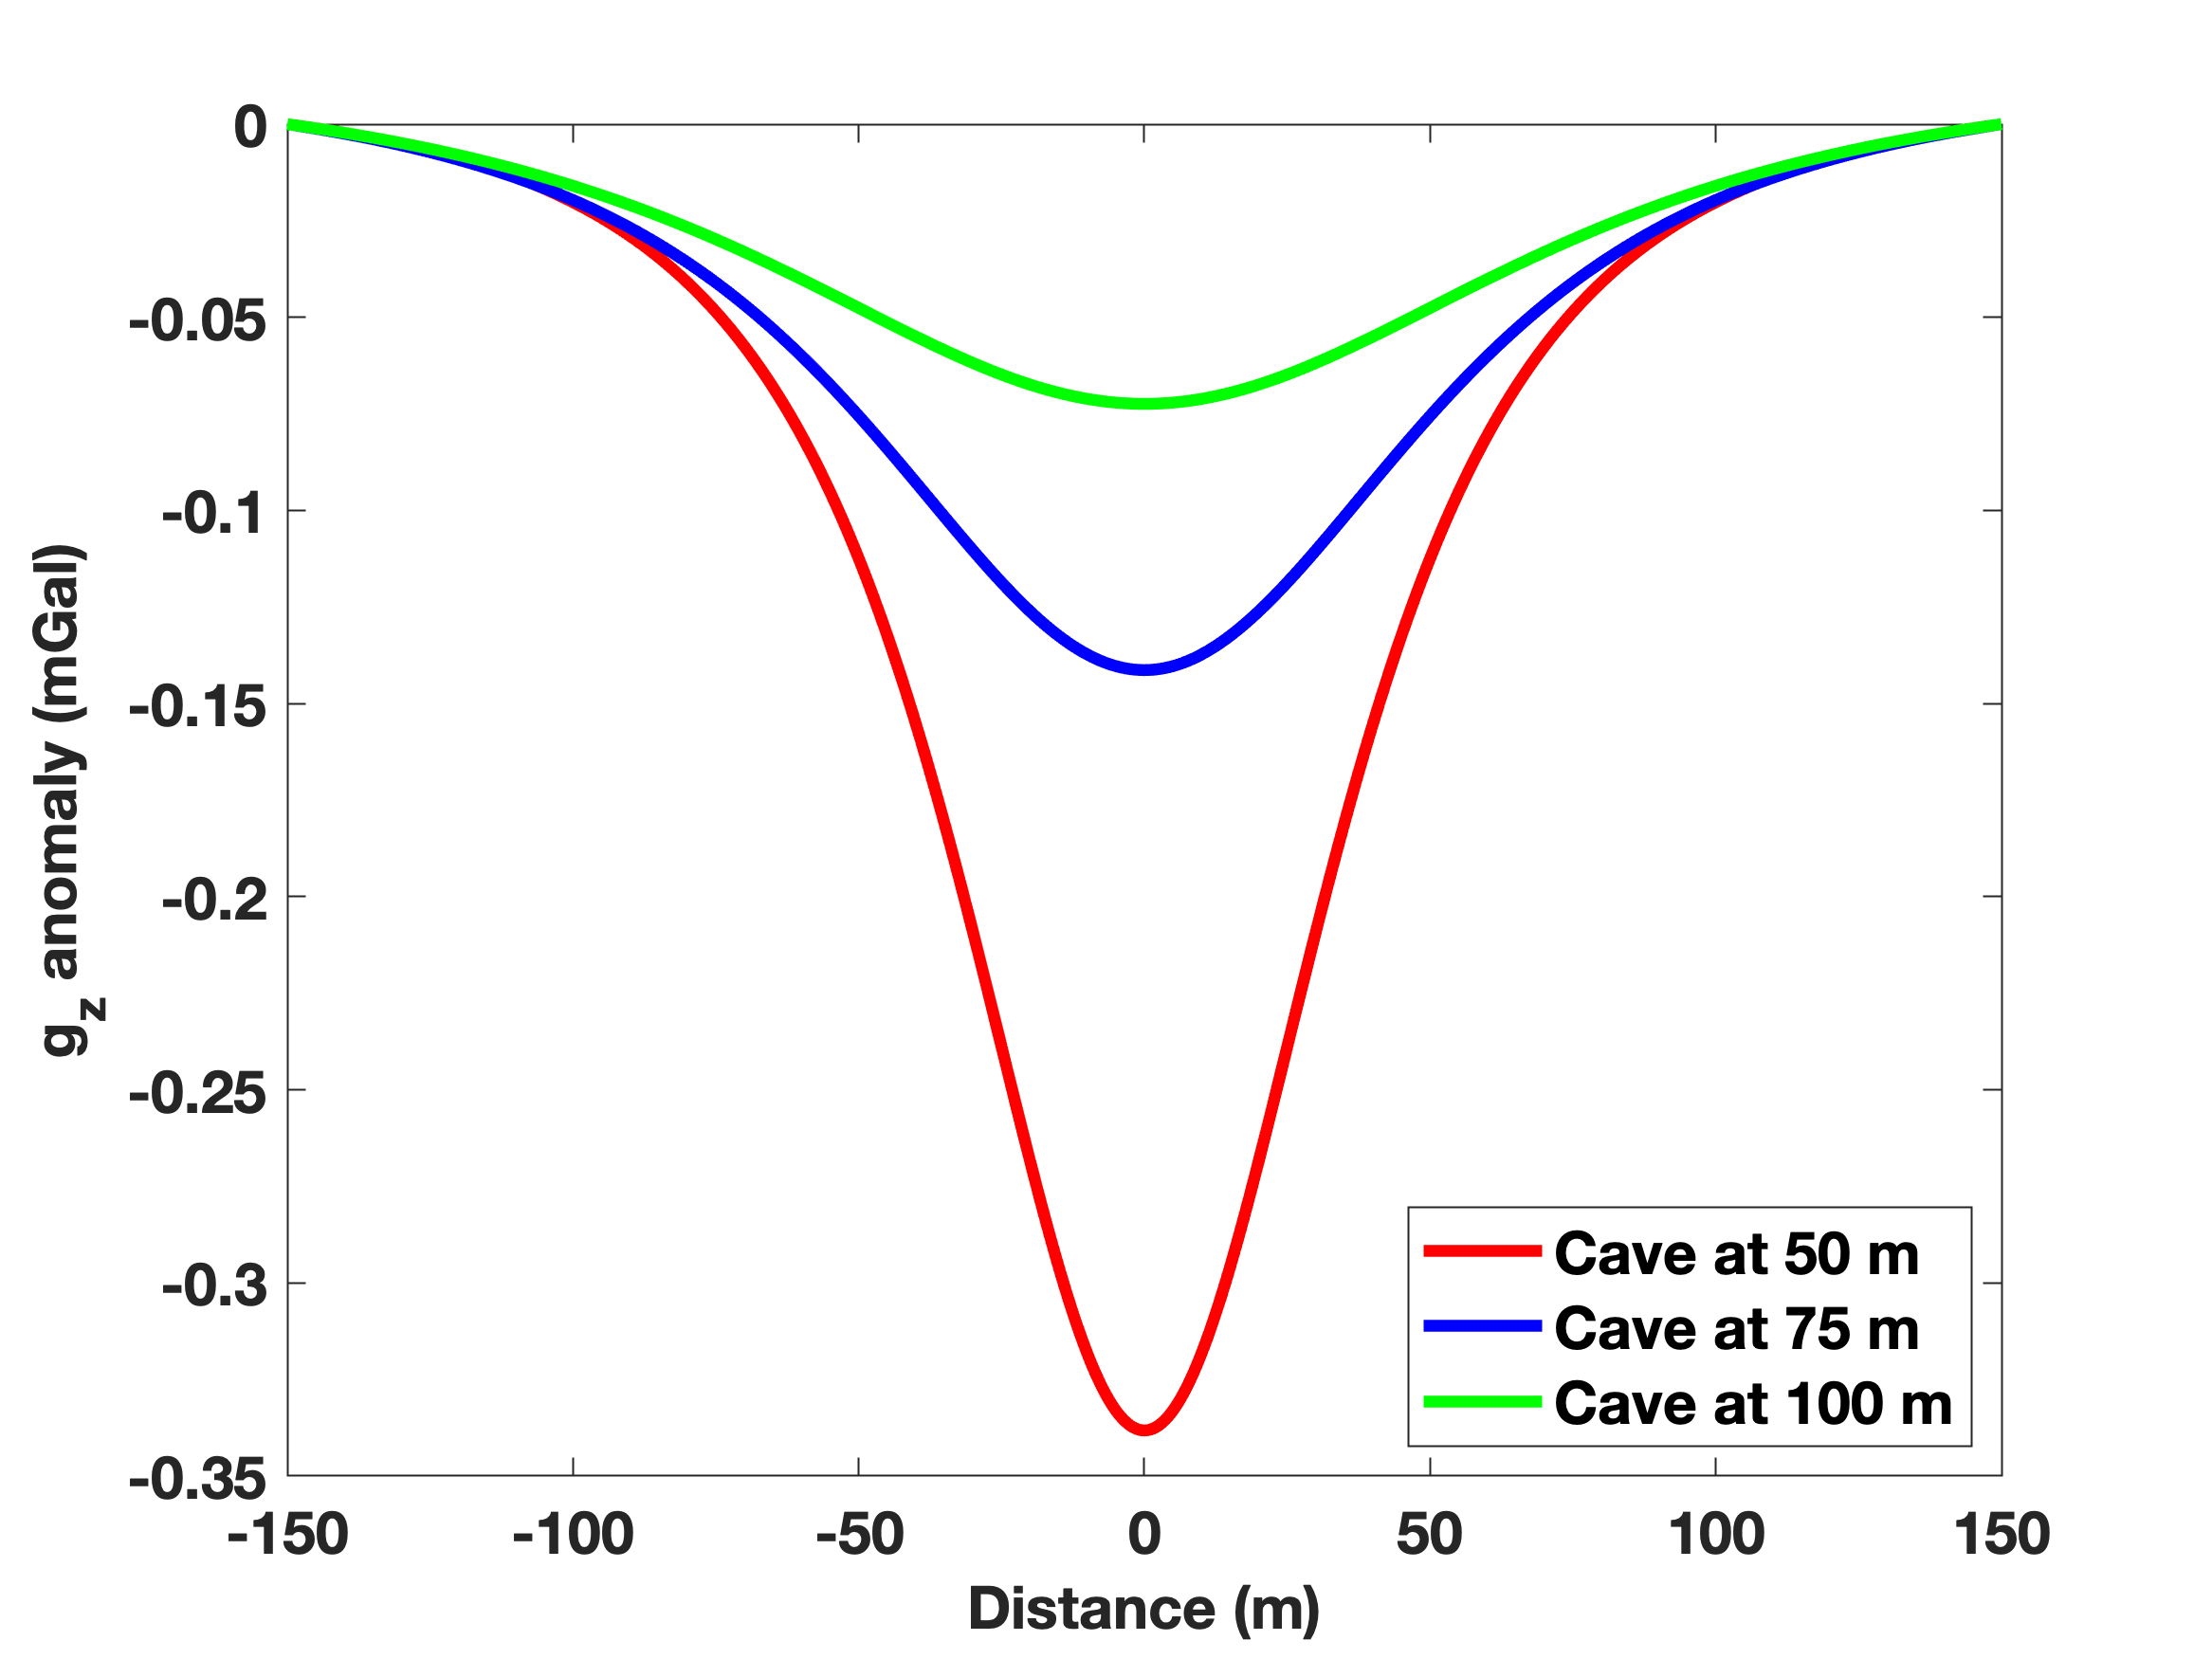
\includegraphics[width=0.5\textwidth]{../GravityAnomaly.png}
% \end{center}

% \noindent\textbf{(c)} We now investigate what information can be gained from the half-width of this anomaly. For this you have to derive an expression that links the half-width of the anomaly (i.e. $g_z = \frac{1}{2}g_{z,max}$ for $x=x_{\frac{1}{2}}$) to the depth of the object. Use this relationship and see if you can infer the depth of the object using the halfwidth. Why could such a relationship be useful?


% \noindent\fcolorbox{myblue}{lightgray}{\parbox{\textwidth}{
% \textbf{Solution:}
% \begin{align*}
% g_z &=\frac{1}{2}g_{z,max} \\
% \rightarrow \frac{z}{(x_{\frac{1}{2}}+z^2)^\frac{3}{2}} &= \frac{1}{2z^2}\\
% \rightarrow \frac{z^3}{(x_{\frac{1}{2}}+z^2)^\frac{3}{2}}&= \frac{1}{2}\\
% \rightarrow \frac{1}{(\frac{x_{\frac{1}{2}}}{z^2}+1)^\frac{3}{2}}&= \frac{1}{2}\\
% \rightarrow z = \frac{x}{\sqrt{2^{\frac{3}{2}}-1}}\approx 0.766 x
% \end{align*}
% }}
% \subsection{Potential of an infite plate (Bouger plate)}




\end{document}